\documentclass[10pt,a4paper]{article}
\usepackage[T1]{fontenc}
\usepackage[utf8]{inputenc}
\usepackage{lmodern,amsmath,booktabs,array,geometry,microtype,xcolor,pgfplots,fancyhdr,hyperref}
\usepackage{caption,multicol,float,titlesec}
\captionsetup{font=small,skip=4pt}
\geometry{margin=13mm}
\pgfplotsset{compat=1.18}
\hypersetup{colorlinks=true,linkcolor=black,urlcolor=blue,citecolor=black,
 pdftitle={Heart Disease Classification: A Reproducible Comparison},
 pdfauthor={Omar Berrada, Othmane Housni, Ali El Azdi}}
\definecolor{accent}{RGB}{26,78,112}
\pagestyle{fancy}\fancyhf{}\fancyhead[L]{\small Heart Disease Classification}
\fancyhead[R]{\small EPFL / CS-233}\fancyfoot[C]{\thepage}
\setlength{\headheight}{14pt}\setlength{\parindent}{0pt}\setlength{\parskip}{3pt}
\setlength{\columnsep}{6mm}
\titlespacing*{\section}{0pt}{9pt}{4pt}
\titlespacing*{\subsection}{0pt}{7pt}{3pt}
\titleformat{\section}{\normalsize\bfseries}{\thesection}{0.7em}{}
\titleformat{\subsection}{\small\bfseries}{\thesubsection}{0.7em}{}
\newcommand{\method}[1]{\textbf{#1}}
% BEGIN GENERATED SUMMARY
% Numerical content generated by scripts/sync_report.py; do not edit marked blocks by hand.
% END GENERATED SUMMARY
\begin{document}
\begin{center}
{\LARGE\bfseries Heart Disease Classification}\\[5pt]
{\large A Reproducible Comparison of Three NumPy Models}\\[7pt]
Omar Berrada \quad Othmane Housni \quad Ali El Azdi\\[3pt]
\small Introduction to Machine Learning (CS-233), EPFL\\
Evaluation date: 6 October 2026
\end{center}
\small
\begin{multicols}{2}

\section{Introduction and data}
We compare distance-weighted K-nearest neighbours (KNN), K-Means with cluster-to-class mapping, and multinomial logistic regression. The objective is to understand their behaviour on a small, imbalanced five-class dataset and to make the evaluation reproducible, rather than to establish a clinical prediction system.

The course dataset derives from the processed Cleveland subset of the UCI Heart Disease dataset~\cite{uci}. Six incomplete records were removed from the original 303 observations. The supplied split contains 237 training records and 60 test records, each with 13 features. Labels range from 0 to 4; label 0 denotes absence of disease. Class counts are $[128,41,30,30,8]$ in training and $[32,13,5,5,5]$ in the fixed test split. The smallest training class contains only eight observations.

\textbf{Fixed-test limitation.} The fixed test split has been used in exploratory logistic-regression parameter searches. Parameter selection in \texttt{evaluate.py} uses training data only. We use nested cross-validation on the 237 training records as the principal comparison and report fixed-test scores as descriptive results. The model families and search ranges were informed by the exploratory experiments, so this comparison remains exploratory.

\section{Methods and preprocessing}
\method{KNN} stores the training samples, computes Euclidean distances, and weights each of the $k$ nearest neighbours by $1/(d+10^{-8})$. A weighted vote determines the predicted label; equal votes are resolved by choosing the smaller label. Odd values of $k$ form our search grid as a practical choice, not a mathematical requirement. Small $k$ can produce a flexible decision rule that is sensitive to noise.

\method{K-Means} starts from $k$ distinct training samples drawn with a fixed seed (42). It alternates nearest-centroid assignment and centroid updates until the centroids stop changing or 500 iterations are reached. After fitting, each cluster is assigned the most common training label among its members. Thus, clustering is unsupervised, but the final cluster-to-class mapping uses labels. Equal class counts favour the smaller label; empty clusters default to label 0. A single fixed initialization is used per fit; no seed is selected by its score.

\method{Logistic regression} uses softmax probabilities for the five classes and full-batch gradient descent. The gradient of the mean cross-entropy is augmented by $\lambda W$, with $\lambda=0.001$. This implementation penalizes all weights, including the bias weights. Parameters start at zero. The learning rate and iteration count are selected by cross-validation; there is no early stopping.

For each fit, means and standard deviations are estimated solely from its training rows. Constant-feature standard deviations are replaced by one. Logistic regression uses all standardized features with a leading bias term. For KNN and K-Means, standardized values are clipped to $[-3,3]$, followed by MinMax scaling using training minima and ranges. This is fixed-threshold clipping, not IQR-based clipping. Constant ranges are replaced by one. Evaluation values need not lie inside $[0,1]$ when they exceed the fitted training range. Features are ranked by their variance after this transformation, and the selected indices are applied to evaluation rows.

Categorical variables retain their supplied numeric encoding. In particular, Euclidean distance imposes an ordering on nominal categories such as chest-pain type. This is a limitation of the course pipeline, not evidence that numeric encoding is optimal.

\section{Validation and parameter selection}
The outer evaluation uses five stratified folds of the training split. For each outer fold, parameters are selected using four stratified inner folds of the remaining training rows. All preprocessing, including feature ranking, is refitted inside every inner fit. The outer validation rows are used only after selection. This separates model selection from performance estimation~\cite{nested,pitfalls}.

Candidate configurations are ranked by mean macro F1, with mean accuracy breaking ties, followed by their declared grid order. We do not choose a validation percentage or a random seed by maximizing its score. All split and model seeds are fixed at 42. The searched configurations are:
\begin{itemize}
\item KNN: $k\in\{1,3,5,7,9,11,15\}$ and retained features $f\in\{7,10,13\}$ (21 configurations).
\item K-Means: $k\in\{5,10,20,30,34,40\}$ and $f\in\{7,10,13\}$ (18 configurations).
\item Logistic regression: learning rate $\eta\in\{0.001,0.01,0.1\}$ and iterations $T\in\{250,500,1000\}$, with fixed $\lambda=0.001$ (9 configurations).
\end{itemize}
After nested evaluation, each method's final configuration is selected by five-fold cross-validation on all 237 training rows and refitted on those rows. Only then is it evaluated on the fixed test split. The majority baseline always predicts the most frequent class of its fitting data.

Accuracy is the percentage of correct predictions. Macro F1 averages the per-class F1 scores equally over the five classes, assigning zero when a class has no true positives. We report the unweighted mean and population standard deviation across the five outer folds. These standard deviations describe fold variation; they are not confidence intervals. The inner search maximum is a selection score and is not treated as an unbiased performance estimate.

\section{Results and interpretation}
\begin{table}[H]
\centering\small
\caption{Principal nested-CV results and descriptive scores on the previously inspected fixed test split. Accuracy is in percent; F1 ranges from 0 to 1. LogReg denotes logistic regression.}
\label{tab:results}
% BEGIN GENERATED RESULTS
\begin{tabular}{@{}lrr@{}}\toprule
\multicolumn{3}{c}{Nested CV: mean $\pm$ SD}\\
Method & Accuracy (\%) & Macro F1\\\midrule
Baseline & $54.02 \pm 0.49$ & $0.140 \pm 0.001$ \\
KNN & $52.37 \pm 6.56$ & $0.279 \pm 0.072$ \\
K-Means & $55.68 \pm 2.39$ & $0.274 \pm 0.043$ \\
LogReg & $56.93 \pm 3.77$ & $0.292 \pm 0.048$ \\
\midrule\multicolumn{3}{c}{Descriptive fixed test}\\
Method & Accuracy (\%) & Macro F1\\\midrule
Baseline & 53.33 & 0.139 \\
KNN & 58.33 & 0.313 \\
K-Means & 60.00 & 0.283 \\
LogReg & 60.00 & 0.287 \\
\bottomrule\end{tabular}
% END GENERATED RESULTS
\end{table}

\begin{table}[H]
\centering\small
\caption{Final configurations selected on training rows only. These configurations can differ from those selected inside individual outer folds.}
\label{tab:params}
\setlength{\tabcolsep}{3pt}\begin{tabular}{@{}ll@{}}\toprule
Method & Selected parameters\\\midrule
% BEGIN GENERATED PARAMETERS
KNN & $k=1$, $f=13$ \\
K-Means & $k=40$, $f=7$ \\
LogReg & $\eta=0.001$, $T=1000$, $\lambda=0.001$ \\
% END GENERATED PARAMETERS
\bottomrule\end{tabular}
\end{table}

% BEGIN GENERATED INTERPRETATION
Logistic regression has the highest mean nested-CV macro F1 in this run (0.292). The three mean scores are close relative to fold variation; this does not establish a reliable ranking. All three methods exceed the majority baseline on mean macro F1, but their absolute scores remain low.
% END GENERATED INTERPRETATION
The baseline is essential: predicting label 0 for every fixed-test record already achieves $32/60=53.33\%$ accuracy, despite poor macro F1. Consequently, accuracy alone would hide substantial differences in performance on minority classes. Appendix~\ref{app:classes} provides per-class results. Differences between the methods should be interpreted cautiously: only eight training records belong to class 4, and each of the three smallest fixed-test classes contains five records.

A higher descriptive test score than a cross-validation score is not, by itself, evidence of either good generalization or overfitting. Averaging test and validation scores does not prevent overfitting. Neither a particular cluster count nor a visual plateau guarantees generalization.

\section{Search behaviour and reproducibility}
Figure~\ref{fig:search} shows training-only selection scores for the distance-based methods. Each curve keeps the feature count fixed. These scores help describe the search; they are not the outer nested-CV estimates in Table~\ref{tab:results}. We do not infer an optimal cluster count from a claimed plateau or choose a model using fixed-test performance.
\begin{figure}[H]
\centering
% BEGIN GENERATED PLOTS
\begin{minipage}{\linewidth}\centering
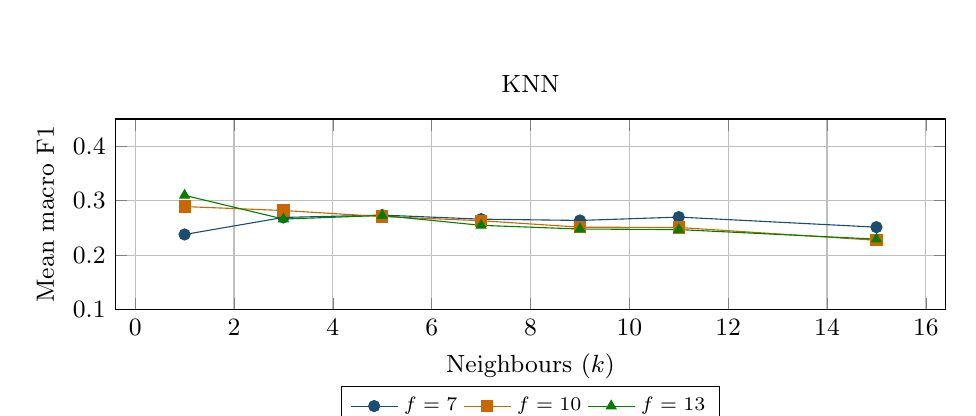
\begin{tikzpicture}
\begin{axis}[width=\linewidth,height=4cm,scale only axis=false,
title={KNN},xlabel={Neighbours ($k$)},ylabel={Mean macro F1},
ymin=0.1,ymax=0.45,grid=major,legend style={font=\scriptsize,at={(0.5,-0.4)},anchor=north,legend columns=3},
tick label style={font=\small},label style={font=\small},title style={font=\small}]
\addplot[color=accent,mark=*] coordinates {(1,0.237823) (3,0.269165) (5,0.273465) (7,0.265997) (9,0.263620) (11,0.269795) (15,0.251265)};
\addlegendentry{$f=7$}
\addplot[color=orange!80!black,mark=square*] coordinates {(1,0.289108) (3,0.281908) (5,0.270745) (7,0.263133) (9,0.251238) (11,0.250718) (15,0.227118)};
\addlegendentry{$f=10$}
\addplot[color=green!50!black,mark=triangle*] coordinates {(1,0.309752) (3,0.266182) (5,0.272759) (7,0.254619) (9,0.247863) (11,0.246837) (15,0.229228)};
\addlegendentry{$f=13$}
\end{axis}\end{tikzpicture}\end{minipage}
\par\medskip
\begin{minipage}{\linewidth}\centering
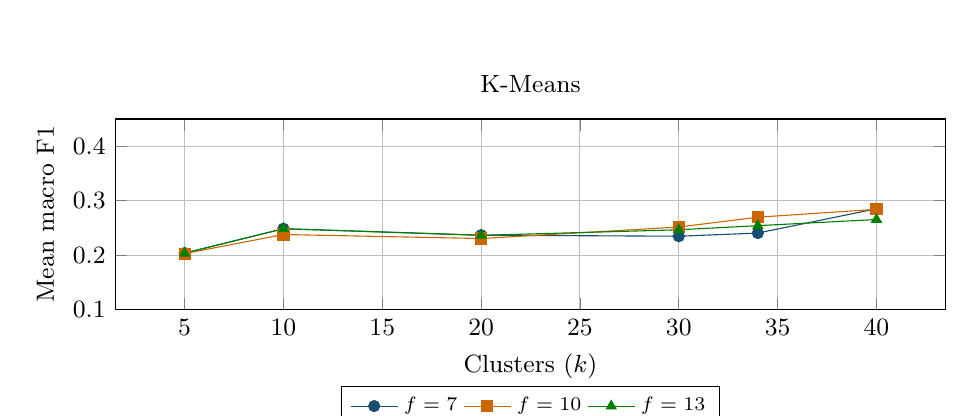
\begin{tikzpicture}
\begin{axis}[width=\linewidth,height=4cm,scale only axis=false,
title={K-Means},xlabel={Clusters ($k$)},ylabel={Mean macro F1},
ymin=0.1,ymax=0.45,grid=major,legend style={font=\scriptsize,at={(0.5,-0.4)},anchor=north,legend columns=3},
tick label style={font=\small},label style={font=\small},title style={font=\small}]
\addplot[color=accent,mark=*] coordinates {(5,0.203631) (10,0.248437) (20,0.236546) (30,0.234611) (34,0.240436) (40,0.285082)};
\addlegendentry{$f=7$}
\addplot[color=orange!80!black,mark=square*] coordinates {(5,0.202695) (10,0.237764) (20,0.230384) (30,0.251504) (34,0.269599) (40,0.284083)};
\addlegendentry{$f=10$}
\addplot[color=green!50!black,mark=triangle*] coordinates {(5,0.203389) (10,0.248404) (20,0.236259) (30,0.246436) (34,0.254031) (40,0.265350)};
\addlegendentry{$f=13$}
\end{axis}\end{tikzpicture}\end{minipage}
% END GENERATED PLOTS
\caption{Mean five-fold macro F1 on the full training split for each searched neighbour or cluster count, with feature count held fixed per curve. All transformations are fitted within each fold.}
\label{fig:search}
\end{figure}

Run \texttt{python evaluate.py} from the repository root to regenerate \path{results/evaluation.json}. The file contains the search grids, dataset checksum, source checksums, NumPy version, selected configurations, outer-fold indices and scores, out-of-fold confusion matrices, and descriptive test predictions. Then run \path{python scripts/sync_report.py} to update the numerical tables and vector plots embedded in this standalone \LaTeX{} source. The README documents installation and PDF compilation.

\section{Experiments and limitations}
The scripts in \texttt{experiments/} explore parameter choices and preprocessing. With their fixed configurations, KNN achieved 68.333\% accuracy and 0.384 macro F1 on the fixed test split; K-Means achieved 60.000\% and 0.277; logistic regression achieved 63.333\% and 0.351. These values come from different preprocessing and model configurations than the nested-CV comparison in Table~\ref{tab:results}.

The exploratory hold-out scores of 68.571\% for KNN and 65.714\% for logistic regression correspond to 15\% validation splits (35 records), while K-Means' 71.154\% corresponds to a 22\% split (52 records). Some exploratory transforms were fitted before the hold-out split, validation proportions were compared by score, and the logistic combined-surface script optimized the average of cross-validation and fixed-test accuracy. These practices can bias the reported performance and are excluded from the selection procedure in \texttt{evaluate.py}.

The study has limited scope. Search ranges are finite, K-Means uses one initialization per fit, nominal features are numerically encoded, and the sample is small and imbalanced. Fold estimates share overlapping training data and should not be read as independent replications. We have not established statistical superiority, causal relationships, or performance on another population. A new external dataset, chosen without consulting its outcomes, would be needed for an independent final evaluation.

\section{Conclusion}
The project provides transparent NumPy implementations and a reproducible comparison that separates training-only parameter selection from outer-fold evaluation. The main finding is limited discrimination across the five classes, especially for rare labels, rather than a universally superior algorithm. Future work could compare categorical encodings, class weighting, alternative feature selection, and multiple K-Means initializations within the same nested validation design. Any confirmatory comparison would require fresh evaluation data and a protocol fixed in advance.

\end{multicols}
\newpage
\appendix
\begin{multicols}{2}
\section{Per-class descriptive test results}\label{app:classes}
The following results use the previously inspected 60-record fixed test split and the final training-selected configurations. Parameter selection in \texttt{evaluate.py} uses training data only. A zero recall means no record of that class was correctly classified; macro averaging retains that class in the score.
\begin{table}[H]
\centering\small
\caption{Recall/F1 pairs by class on the descriptive fixed test split. Support is the number of true records in each class.}
\label{tab:classes}
% BEGIN GENERATED CLASSES
\setlength{\tabcolsep}{2pt}
\begin{tabular}{@{}rr*{3}{r}@{}}\toprule
Class & Support & KNN & K-Means & LogReg\\\midrule
0 & 32 & 0.844/0.844 & 1.000/0.800 & 0.969/0.886 \\
1 & 13 & 0.462/0.500 & 0.154/0.250 & 0.154/0.235 \\
2 & 5 & 0.000/0.000 & 0.400/0.364 & 0.000/0.000 \\
3 & 5 & 0.400/0.222 & 0.000/0.000 & 0.600/0.316 \\
4 & 5 & 0.000/0.000 & 0.000/0.000 & 0.000/0.000 \\
\bottomrule\end{tabular}
% END GENERATED CLASSES
\end{table}

\subsection{Confusion matrices}
Rows are true labels and columns are predicted labels, both ordered 0 to 4. Each matrix contains all 60 fixed-test records. These matrices describe class-specific errors, rather than clustering purity.
\begin{center}
% BEGIN GENERATED CONFUSION
\begin{minipage}{0.48\linewidth}\centering\small\setlength{\tabcolsep}{2pt}
\textbf{KNN}\\[4pt]
\begin{tabular}{@{}r*{5}{r}@{}}\toprule
 & 0 & 1 & 2 & 3 & 4\\\midrule
0 & 27 & 2 & 0 & 2 & 1 \\
1 & 3 & 6 & 0 & 4 & 0 \\
2 & 1 & 2 & 0 & 2 & 0 \\
3 & 1 & 1 & 1 & 2 & 0 \\
4 & 0 & 0 & 2 & 3 & 0 \\
\bottomrule\end{tabular}\end{minipage}
\hfill
\begin{minipage}{0.48\linewidth}\centering\small\setlength{\tabcolsep}{2pt}
\textbf{K-Means}\\[4pt]
\begin{tabular}{@{}r*{5}{r}@{}}\toprule
 & 0 & 1 & 2 & 3 & 4\\\midrule
0 & 32 & 0 & 0 & 0 & 0 \\
1 & 9 & 2 & 2 & 0 & 0 \\
2 & 2 & 0 & 2 & 1 & 0 \\
3 & 2 & 1 & 2 & 0 & 0 \\
4 & 3 & 0 & 0 & 2 & 0 \\
\bottomrule\end{tabular}\end{minipage}
\par\medskip
\begin{minipage}{0.48\linewidth}\centering\small\setlength{\tabcolsep}{2pt}
\textbf{LogReg}\\[4pt]
\begin{tabular}{@{}r*{5}{r}@{}}\toprule
 & 0 & 1 & 2 & 3 & 4\\\midrule
0 & 31 & 0 & 1 & 0 & 0 \\
1 & 7 & 2 & 2 & 2 & 0 \\
2 & 0 & 1 & 0 & 4 & 0 \\
3 & 0 & 1 & 1 & 3 & 0 \\
4 & 0 & 0 & 0 & 5 & 0 \\
\bottomrule\end{tabular}\end{minipage}
% END GENERATED CONFUSION
\end{center}

\subsection{Data attribution}
The original dataset is attributed to Andras Janosi, William Steinbrunn, Matthias Pfisterer, and Robert Detrano and is distributed under CC BY 4.0~\cite{uci}. The course adaptation removes incomplete records and supplies the fixed split. The dataset checksum is recorded in the generated JSON to identify this exact adaptation.

\begin{thebibliography}{9}\small
\bibitem{uci} A. Janosi, W. Steinbrunn, M. Pfisterer, and R. Detrano. \emph{Heart Disease}. UCI Machine Learning Repository, 1989. DOI: \href{https://doi.org/10.24432/C52P4X}{10.24432/C52P4X}. License: \href{https://creativecommons.org/licenses/by/4.0/}{CC BY 4.0}.
\bibitem{nested} Scikit-learn developers. \emph{Nested versus non-nested cross-validation}. \href{https://scikit-learn.org/stable/auto_examples/model_selection/plot_nested_cross_validation_iris.html}{Online documentation}. Accessed 6 October 2026. Methodological reference; scikit-learn is not a runtime dependency.
\bibitem{pitfalls} Scikit-learn developers. \emph{Common pitfalls and recommended practices}. \href{https://scikit-learn.org/stable/common_pitfalls.html}{Online documentation}. Accessed 6 October 2026.
\end{thebibliography}
\end{multicols}
\end{document}
